\documentclass[11pt]{article}

\usepackage{fullpage} 
\usepackage{hyperref}
\usepackage{amsmath}
\usepackage{amssymb}
\usepackage{amsthm}
\usepackage{graphicx}
\usepackage{pgf}
\usepackage{tikz}
\usetikzlibrary{arrows,automata}

\usepackage{indentfirst}

\newcommand{\question}[2] {\vspace{0.3in}\noindent{\subsection*{Question #1. #2} \vspace{0.15in}}}

\renewcommand{\part}[1] {{\vspace{0.15in}\noindent\textbf (#1)} \vspace{0.10in}}



%  ----------------------------------------------------------------
%                         Start here
% ----------------------------------------------------------------
 
\begin{document}

\title{Assignment \#5} %Replace X with the appropriate number
\author{\Large Gustavo Estrela de Matos\\ %Replace with your name
CSCE 433: Formal Languages and Automata} %If necessary, replace with your course number and title
\date{\today} 

\maketitle

\question{1}{For each of the following languages, construct a PDA to accept $L$. \\
\part{a} $L = \{a^n b^{2n} \mid n \geq 0\}$ \\
\part{b} $L = \{a^ib^jc^k \mid i, j, k \geq 0$ and $i + k = j\}$ \\
\part{c} $L = \{w \mid w$ has twice as many $0$'s as $1$'s$\}$}

\part{a}

The idea for this language PDA is to have a state where the $a$'s are read and for each of them we push $2$ elements in the stack; and a also a state where the $b$'s are read and for each of them an element is poped from the stack. Since we pushed $2$ elements for every $a$ and poped one for every $b$ we can guarantee that when the stack has $z_0$ on the top.

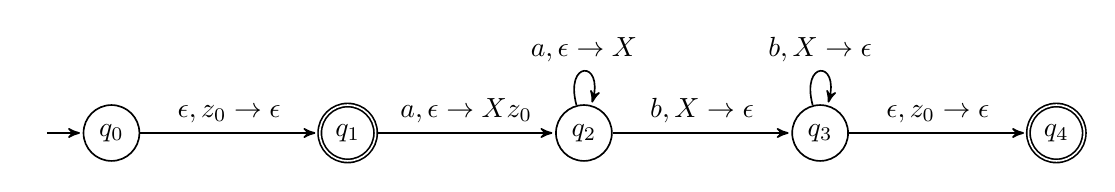
\begin{tikzpicture}[->,>=stealth',shorten >=1pt,auto,node distance=3cm, semithick, initial text={}, align=left]
  
    \tikzstyle{every state}=[fill=white,draw=black,text=black, minimum size=15pt]

    \node[initial,state]    (0)              {$q_0$};
    \node[accepting, state] (1) [right of=0] {$q_1$};
    \node[state]            (2) [right of=1] {$q_2$};
    \node[state]            (3) [right of=2] {$q_3$};
    \node[state, accepting] (4) [right of=3] {$q_4$};
 
    \path (0) edge node {$\epsilon, z_0 \rightarrow \epsilon$}     (1)
          (1) edge node {$a, \epsilon \rightarrow Xz_0$}           (2)
          (2) edge [loop above] node {$a, \epsilon \rightarrow X$} (2)
          (2) edge node {$b, X \rightarrow \epsilon$}              (3)
          (3) edge [loop above] node {$b, X \rightarrow \epsilon$} (3)
          (3) edge node {$\epsilon, z_0 \rightarrow \epsilon$}     (4)
    ;                      
\end{tikzpicture}    

This PDA is deterministic.


\part{b}

Saying that $i + k = j$ is the same as saying that $k = j - i$, therefore we need to calculate $j- i$ while reading $a$s and $b$s. To do that we are going to push an element $X$ for every $a$ and pop them for every $b$ read. Once the stack have $z_0$ on the top we can start pushing $Y$s for every $b$ read. 

The number of $Y$s in the stack after reading all $b$s will be the number of $c$s needed to the input to be in $L$. If after reading all the $b$s we have a $X$ on the top of the stack we know we already know that the string is not in $L$ because having a $X$ on the top means that $j < i$ thus there's no positive $k$ such that $i + k = j$.

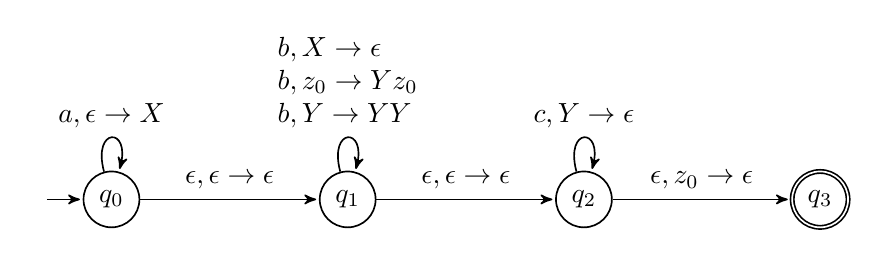
\begin{tikzpicture}[->,>=stealth',shorten >=1pt,auto,node distance=3cm, semithick, initial text={}, align=left]
  
    \tikzstyle{every state}=[fill=white,draw=black,text=black, minimum size=15pt]

    \node[initial,state]    (0)              {$q_0$};
    \node[state]            (1) [right of=0] {$q_1$};
    \node[state]            (2) [right of=1] {$q_2$};
    \node[state, accepting] (3) [right of=2] {$q_3$};
 
    \path (0) edge node {$\epsilon,\epsilon \rightarrow \epsilon$} (1)
          (0) edge [loop above] node {$a,\epsilon \rightarrow X$}  (1)
          (1) edge node {$\epsilon, \epsilon \rightarrow \epsilon$}(2)
          (1) edge [loop above] node {$b, X \rightarrow \epsilon$ \\ 
                                      $b, z_0 \rightarrow Yz_0$   \\
                                      $b, Y \rightarrow YY$}       (1)
          (2) edge [loop above] node {$c, Y \rightarrow \epsilon$} (2)
          (2) edge node {$\epsilon, z_0 \rightarrow \epsilon$}(3)
    ;                      
\end{tikzpicture}    

This PDA is nondeterministic.

\part{c}

To build this DFA we are going to use two symbols:
\begin{itemize}
    \item{$Y$:} the number of $Y$s in the stack will represent the number of $0$s needed for the string to be in $L$;
    \item{$X$:} the number of $X$s in the stack will represent the number of $1$s needed for the string to be in $L$; \\
and the stack will keep the stack with only $z_0$ and either $X$s or $Y$s.
\end{itemize}

Our DFA will have at least two states: one to represent that the string so far read is in $L$ and other state if there are symbols needed to be read for the string to be in $L$. If we are in the second state we need to have a feew rules:
\begin{itemize}
\item{$1, Y \rightarrow YYY$:} if needed $0$s and read a $1$ we need two more $0$.
\item{$0, Y \rightarrow \epsilon$:} if needed $0$s and read a $0$ we need one less $0$.
\item{$1, X \rightarrow \epsilon$:} if needed $1$s and read a $1$ we need one less $1$.
\end{itemize}

But what if we read one more $0$ when needing $1$s? We would need to read one more $1$ and one more $0$. Since we don't want to have mixed $X$s and $Y$s in our stack we will create another state that will represent our need for an amount of $1$s and one more $0$. From this state three things can happen:
\begin{itemize}
    \item{$1, X \rightarrow \epsilon$:} if we read a $1$ we would need one less $1$;
    \item{$\epsilon, z_0 \rightarrow Xz_0$:} if we read all $1$s we needed, then we only need to read one more $0$;
    \item{$0, X \rightarrow XX$:} if we read a $0$ then we only need to read one more $1$ (for the $0$ we read when entering and getting out of this state).
\end{itemize}

Finally, the PDA:


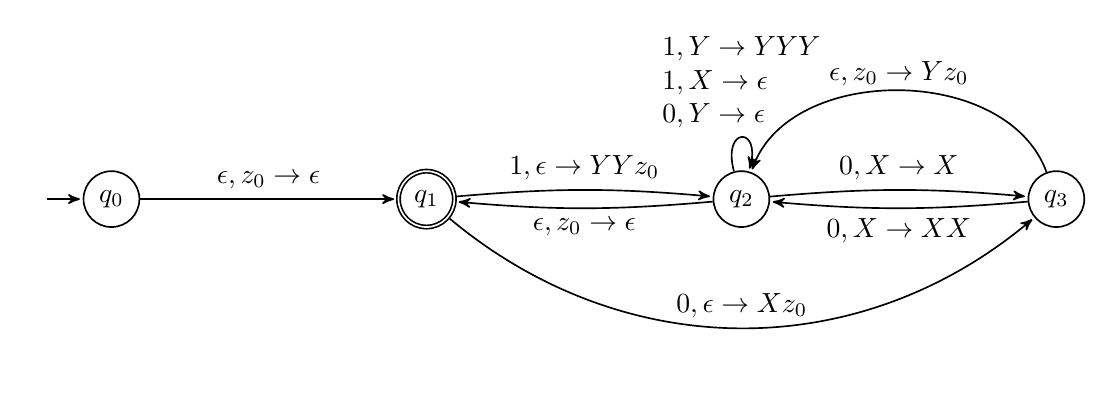
\begin{tikzpicture}[->,>=stealth',shorten >=1pt,auto,node distance=4cm, semithick, initial text={}, align=left]
  
    \tikzstyle{every state}=[fill=white,draw=black,text=black, minimum size=15pt]

    \node[initial,state]    (0)              {$q_0$};
    \node[state, accepting] (1) [right of=0] {$q_1$};
    \node[state]            (2) [right of=1] {$q_2$};
    \node[state]            (3) [right of=2] {$q_3$};
 
    \path (0) edge node {$\epsilon, z_0 \rightarrow \epsilon$}      (1)
          (1) edge [bend left = 5] node {$1, \epsilon \rightarrow YYz_0$} (2)
          (1) edge [bend right = 40] node {$0, \epsilon \rightarrow Xz_0$} (3)
          (2) edge [bend left = 5] node {$\epsilon, z_0 \rightarrow \epsilon$} (1)
          (2) edge [loop above] node {$1, Y \rightarrow YYY$ \\
                                      $1, X \rightarrow \epsilon$ \\
                                      $0, Y \rightarrow \epsilon$} (2)
          (2) edge [bend left = 5] node {$0, X \rightarrow X$} (3)
          (3) edge [bend left = 5] node {$0, X \rightarrow XX$} (2)
          (3) edge [bend right = 70] node [yshift = 5mm] {$\epsilon, z_0 \rightarrow Yz_0$} (2)
    ;                      
\end{tikzpicture}    


\question{2}{}
\question{3}{}
\question{4}{}

\end{document}
